% Created by tikzDevice version 0.12.6 on 2025-01-26 19:10:08
% !TEX encoding = UTF-8 Unicode
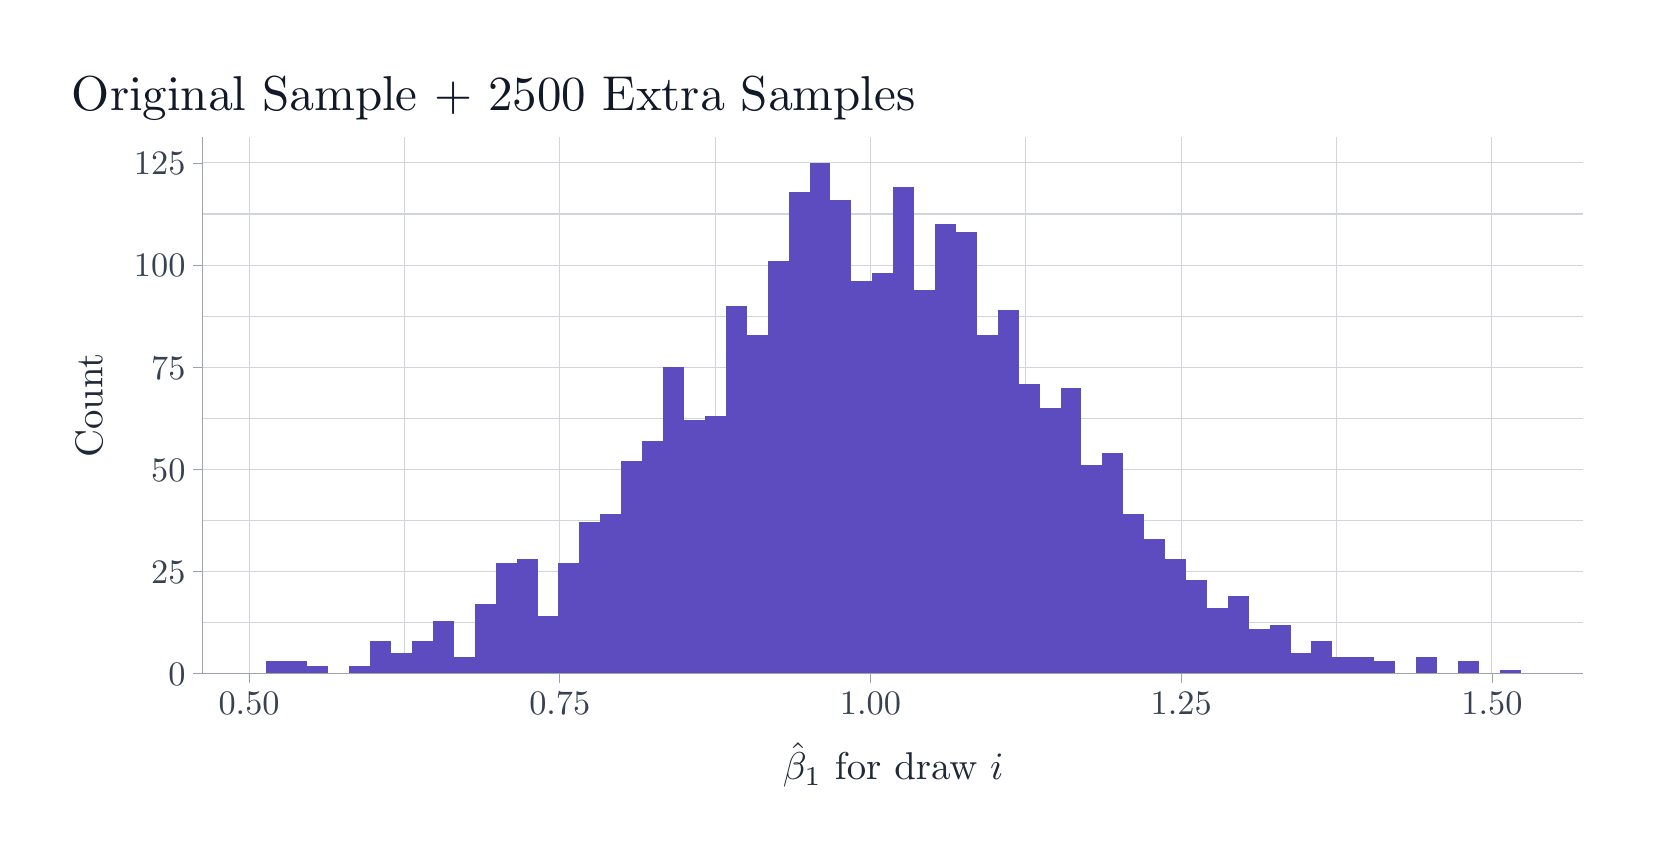
\begin{tikzpicture}[x=1pt,y=1pt]
\definecolor{fillColor}{RGB}{255,255,255}
\path[use as bounding box,fill=fillColor] (0,0) rectangle (578.16,289.08);
\begin{scope}
\path[clip] (  0.00,  0.00) rectangle (578.16,289.08);
\definecolor{drawColor}{RGB}{255,255,255}

\path[draw=drawColor,line width= 0.7pt,line join=round,line cap=round,fill=fillColor] (  0.00,  0.00) rectangle (578.16,289.08);
\end{scope}
\begin{scope}
\path[clip] ( 63.32, 55.65) rectangle (562.16,249.43);
\definecolor{drawColor}{RGB}{255,255,255}
\definecolor{fillColor}{RGB}{255,255,255}

\path[draw=drawColor,line width= 0.7pt,line join=round,line cap=round,fill=fillColor] ( 63.32, 55.65) rectangle (562.16,249.43);
\definecolor{drawColor}{RGB}{209,213,219}

\path[draw=drawColor,line width= 0.4pt,line join=round] ( 63.32, 74.10) --
	(562.16, 74.10);

\path[draw=drawColor,line width= 0.4pt,line join=round] ( 63.32,111.02) --
	(562.16,111.02);

\path[draw=drawColor,line width= 0.4pt,line join=round] ( 63.32,147.93) --
	(562.16,147.93);

\path[draw=drawColor,line width= 0.4pt,line join=round] ( 63.32,184.84) --
	(562.16,184.84);

\path[draw=drawColor,line width= 0.4pt,line join=round] ( 63.32,221.75) --
	(562.16,221.75);

\path[draw=drawColor,line width= 0.4pt,line join=round] (136.15, 55.65) --
	(136.15,249.43);

\path[draw=drawColor,line width= 0.4pt,line join=round] (248.42, 55.65) --
	(248.42,249.43);

\path[draw=drawColor,line width= 0.4pt,line join=round] (360.69, 55.65) --
	(360.69,249.43);

\path[draw=drawColor,line width= 0.4pt,line join=round] (472.96, 55.65) --
	(472.96,249.43);

\path[draw=drawColor,line width= 0.4pt,line join=round] ( 63.32, 55.65) --
	(562.16, 55.65);

\path[draw=drawColor,line width= 0.4pt,line join=round] ( 63.32, 92.56) --
	(562.16, 92.56);

\path[draw=drawColor,line width= 0.4pt,line join=round] ( 63.32,129.47) --
	(562.16,129.47);

\path[draw=drawColor,line width= 0.4pt,line join=round] ( 63.32,166.38) --
	(562.16,166.38);

\path[draw=drawColor,line width= 0.4pt,line join=round] ( 63.32,203.29) --
	(562.16,203.29);

\path[draw=drawColor,line width= 0.4pt,line join=round] ( 63.32,240.20) --
	(562.16,240.20);

\path[draw=drawColor,line width= 0.4pt,line join=round] ( 80.01, 55.65) --
	( 80.01,249.43);

\path[draw=drawColor,line width= 0.4pt,line join=round] (192.28, 55.65) --
	(192.28,249.43);

\path[draw=drawColor,line width= 0.4pt,line join=round] (304.55, 55.65) --
	(304.55,249.43);

\path[draw=drawColor,line width= 0.4pt,line join=round] (416.82, 55.65) --
	(416.82,249.43);

\path[draw=drawColor,line width= 0.4pt,line join=round] (529.10, 55.65) --
	(529.10,249.43);
\definecolor{fillColor}{RGB}{92,76,191}

\path[fill=fillColor] ( 85.99, 55.65) rectangle ( 93.55, 60.08);

\path[fill=fillColor] ( 93.55, 55.65) rectangle (101.11, 60.08);

\path[fill=fillColor] (101.11, 55.65) rectangle (108.67, 58.60);

\path[fill=fillColor] (108.67, 55.65) rectangle (116.23, 55.65);

\path[fill=fillColor] (116.23, 55.65) rectangle (123.78, 58.60);

\path[fill=fillColor] (123.78, 55.65) rectangle (131.34, 67.46);

\path[fill=fillColor] (131.34, 55.65) rectangle (138.90, 63.03);

\path[fill=fillColor] (138.90, 55.65) rectangle (146.46, 67.46);

\path[fill=fillColor] (146.46, 55.65) rectangle (154.02, 74.84);

\path[fill=fillColor] (154.02, 55.65) rectangle (161.58, 61.56);

\path[fill=fillColor] (161.58, 55.65) rectangle (169.13, 80.75);

\path[fill=fillColor] (169.13, 55.65) rectangle (176.69, 95.51);

\path[fill=fillColor] (176.69, 55.65) rectangle (184.25, 96.99);

\path[fill=fillColor] (184.25, 55.65) rectangle (191.81, 76.32);

\path[fill=fillColor] (191.81, 55.65) rectangle (199.37, 95.51);

\path[fill=fillColor] (199.37, 55.65) rectangle (206.92,110.28);

\path[fill=fillColor] (206.92, 55.65) rectangle (214.48,113.23);

\path[fill=fillColor] (214.48, 55.65) rectangle (222.04,132.42);

\path[fill=fillColor] (222.04, 55.65) rectangle (229.60,139.81);

\path[fill=fillColor] (229.60, 55.65) rectangle (237.16,166.38);

\path[fill=fillColor] (237.16, 55.65) rectangle (244.72,147.19);

\path[fill=fillColor] (244.72, 55.65) rectangle (252.27,148.66);

\path[fill=fillColor] (252.27, 55.65) rectangle (259.83,188.53);

\path[fill=fillColor] (259.83, 55.65) rectangle (267.39,178.19);

\path[fill=fillColor] (267.39, 55.65) rectangle (274.95,204.77);

\path[fill=fillColor] (274.95, 55.65) rectangle (282.51,229.87);

\path[fill=fillColor] (282.51, 55.65) rectangle (290.06,240.20);

\path[fill=fillColor] (290.06, 55.65) rectangle (297.62,226.92);

\path[fill=fillColor] (297.62, 55.65) rectangle (305.18,197.39);

\path[fill=fillColor] (305.18, 55.65) rectangle (312.74,200.34);

\path[fill=fillColor] (312.74, 55.65) rectangle (320.30,231.34);

\path[fill=fillColor] (320.30, 55.65) rectangle (327.86,194.43);

\path[fill=fillColor] (327.86, 55.65) rectangle (335.41,218.06);

\path[fill=fillColor] (335.41, 55.65) rectangle (342.97,215.10);

\path[fill=fillColor] (342.97, 55.65) rectangle (350.53,178.19);

\path[fill=fillColor] (350.53, 55.65) rectangle (358.09,187.05);

\path[fill=fillColor] (358.09, 55.65) rectangle (365.65,160.48);

\path[fill=fillColor] (365.65, 55.65) rectangle (373.21,151.62);

\path[fill=fillColor] (373.21, 55.65) rectangle (380.76,159.00);

\path[fill=fillColor] (380.76, 55.65) rectangle (388.32,130.95);

\path[fill=fillColor] (388.32, 55.65) rectangle (395.88,135.38);

\path[fill=fillColor] (395.88, 55.65) rectangle (403.44,113.23);

\path[fill=fillColor] (403.44, 55.65) rectangle (411.00,104.37);

\path[fill=fillColor] (411.00, 55.65) rectangle (418.55, 96.99);

\path[fill=fillColor] (418.55, 55.65) rectangle (426.11, 89.61);

\path[fill=fillColor] (426.11, 55.65) rectangle (433.67, 79.27);

\path[fill=fillColor] (433.67, 55.65) rectangle (441.23, 83.70);

\path[fill=fillColor] (441.23, 55.65) rectangle (448.79, 71.89);

\path[fill=fillColor] (448.79, 55.65) rectangle (456.35, 73.37);

\path[fill=fillColor] (456.35, 55.65) rectangle (463.90, 63.03);

\path[fill=fillColor] (463.90, 55.65) rectangle (471.46, 67.46);

\path[fill=fillColor] (471.46, 55.65) rectangle (479.02, 61.56);

\path[fill=fillColor] (479.02, 55.65) rectangle (486.58, 61.56);

\path[fill=fillColor] (486.58, 55.65) rectangle (494.14, 60.08);

\path[fill=fillColor] (494.14, 55.65) rectangle (501.69, 55.65);

\path[fill=fillColor] (501.69, 55.65) rectangle (509.25, 61.56);

\path[fill=fillColor] (509.25, 55.65) rectangle (516.81, 55.65);

\path[fill=fillColor] (516.81, 55.65) rectangle (524.37, 60.08);

\path[fill=fillColor] (524.37, 55.65) rectangle (531.93, 55.65);

\path[fill=fillColor] (531.93, 55.65) rectangle (539.49, 57.13);
\end{scope}
\begin{scope}
\path[clip] (  0.00,  0.00) rectangle (578.16,289.08);
\definecolor{drawColor}{RGB}{156,163,175}

\path[draw=drawColor,line width= 0.3pt,line join=round] ( 63.32, 55.65) --
	( 63.32,249.43);
\end{scope}
\begin{scope}
\path[clip] (  0.00,  0.00) rectangle (578.16,289.08);
\definecolor{drawColor}{RGB}{55,65,81}

\node[text=drawColor,anchor=base east,inner sep=0pt, outer sep=0pt, scale=  1.24] at ( 57.02, 51.37) {0};

\node[text=drawColor,anchor=base east,inner sep=0pt, outer sep=0pt, scale=  1.24] at ( 57.02, 88.28) {25};

\node[text=drawColor,anchor=base east,inner sep=0pt, outer sep=0pt, scale=  1.24] at ( 57.02,125.19) {50};

\node[text=drawColor,anchor=base east,inner sep=0pt, outer sep=0pt, scale=  1.24] at ( 57.02,162.10) {75};

\node[text=drawColor,anchor=base east,inner sep=0pt, outer sep=0pt, scale=  1.24] at ( 57.02,199.01) {100};

\node[text=drawColor,anchor=base east,inner sep=0pt, outer sep=0pt, scale=  1.24] at ( 57.02,235.92) {125};
\end{scope}
\begin{scope}
\path[clip] (  0.00,  0.00) rectangle (578.16,289.08);
\definecolor{drawColor}{RGB}{156,163,175}

\path[draw=drawColor,line width= 0.3pt,line join=round] ( 59.82, 55.65) --
	( 63.32, 55.65);

\path[draw=drawColor,line width= 0.3pt,line join=round] ( 59.82, 92.56) --
	( 63.32, 92.56);

\path[draw=drawColor,line width= 0.3pt,line join=round] ( 59.82,129.47) --
	( 63.32,129.47);

\path[draw=drawColor,line width= 0.3pt,line join=round] ( 59.82,166.38) --
	( 63.32,166.38);

\path[draw=drawColor,line width= 0.3pt,line join=round] ( 59.82,203.29) --
	( 63.32,203.29);

\path[draw=drawColor,line width= 0.3pt,line join=round] ( 59.82,240.20) --
	( 63.32,240.20);
\end{scope}
\begin{scope}
\path[clip] (  0.00,  0.00) rectangle (578.16,289.08);
\definecolor{drawColor}{RGB}{156,163,175}

\path[draw=drawColor,line width= 0.3pt,line join=round] ( 63.32, 55.65) --
	(562.16, 55.65);
\end{scope}
\begin{scope}
\path[clip] (  0.00,  0.00) rectangle (578.16,289.08);
\definecolor{drawColor}{RGB}{156,163,175}

\path[draw=drawColor,line width= 0.3pt,line join=round] ( 80.01, 52.15) --
	( 80.01, 55.65);

\path[draw=drawColor,line width= 0.3pt,line join=round] (192.28, 52.15) --
	(192.28, 55.65);

\path[draw=drawColor,line width= 0.3pt,line join=round] (304.55, 52.15) --
	(304.55, 55.65);

\path[draw=drawColor,line width= 0.3pt,line join=round] (416.82, 52.15) --
	(416.82, 55.65);

\path[draw=drawColor,line width= 0.3pt,line join=round] (529.10, 52.15) --
	(529.10, 55.65);
\end{scope}
\begin{scope}
\path[clip] (  0.00,  0.00) rectangle (578.16,289.08);
\definecolor{drawColor}{RGB}{55,65,81}

\node[text=drawColor,anchor=base,inner sep=0pt, outer sep=0pt, scale=  1.24] at ( 80.01, 40.78) {0.50};

\node[text=drawColor,anchor=base,inner sep=0pt, outer sep=0pt, scale=  1.24] at (192.28, 40.78) {0.75};

\node[text=drawColor,anchor=base,inner sep=0pt, outer sep=0pt, scale=  1.24] at (304.55, 40.78) {1.00};

\node[text=drawColor,anchor=base,inner sep=0pt, outer sep=0pt, scale=  1.24] at (416.82, 40.78) {1.25};

\node[text=drawColor,anchor=base,inner sep=0pt, outer sep=0pt, scale=  1.24] at (529.10, 40.78) {1.50};
\end{scope}
\begin{scope}
\path[clip] (  0.00,  0.00) rectangle (578.16,289.08);
\definecolor{drawColor}{RGB}{31,41,55}

\node[text=drawColor,anchor=base,inner sep=0pt, outer sep=0pt, scale=  1.40] at (312.74, 17.36) {$\hat{\beta}_1$ for draw $i$};
\end{scope}
\begin{scope}
\path[clip] (  0.00,  0.00) rectangle (578.16,289.08);
\definecolor{drawColor}{RGB}{31,41,55}

\node[text=drawColor,rotate= 90.00,anchor=base,inner sep=0pt, outer sep=0pt, scale=  1.40] at ( 27.00,152.54) {Count};
\end{scope}
\begin{scope}
\path[clip] (  0.00,  0.00) rectangle (578.16,289.08);
\definecolor{drawColor}{RGB}{17,24,39}

\node[text=drawColor,anchor=base west,inner sep=0pt, outer sep=0pt, scale=  1.77] at ( 16.00,259.15) {Original Sample + 2500 Extra Samples};
\end{scope}
\end{tikzpicture}
